%%%%%%%%%%%%%%%%%%%%%%%%%%%%%%%%%%%%%%%%%%%%%%%%%%%%%%%%%%%%%%%%%%%%%%%%%%%%%%%%
%2345678901234567890123456789012345678901234567890123456789012345678901234567890
%        1         2         3         4         5         6         7         8

\documentclass[letterpaper, 10 pt, conference]{ieeeconf}  % Comment this line out if you need a4paper

%\documentclass[a4paper, 10pt, conference]{ieeeconf}      % Use this line for a4 paper

\IEEEoverridecommandlockouts                              % This command is only needed if 
                                                          % you want to use the \thanks command

\overrideIEEEmargins                                      % Needed to meet printer requirements.

% See the \addtolength command later in the file to balance the column lengths
% on the last page of the document

% The following packages can be found on http:\\www.ctan.org
\usepackage{graphicx} % for pdf, bitmapped graphics files
\graphicspath{ {images/} }
%\usepackage{epsfig} % for postscript graphics files
%\usepackage{mathptmx} % assumes new font selection scheme installed
%\usepackage{times} % assumes new font selection scheme installed
%\usepackage{amsmath} % assumes amsmath package installed
%\usepackage{amssymb}  % assumes amsmath package installed
\usepackage{booktabs}
\usepackage{multirow}

\title{\LARGE \bf
HW4: Game Theory\\
ROB538
}


\author{Ammar Kothari$^{1}$% <-this % stops a space
\thanks{$^{1}$Kothari  is with graduate students at Oregon State University in the Robotics Department
        {\tt\small KothariA@OregonState.edu}}%
}


\begin{document}



\maketitle
\thispagestyle{empty}
\pagestyle{empty}


%%%%%%%%%%%%%%%%%%%%%%%%%%%%%%%%%%%%%%%%%%%%%%%%%%%%%%%%%%%%%%%%%%%%%%%%%%%%%%%%
% \begin{abstract}

% \end{abstract}
%%%%%%%%%%%%%%%%%%%%%%%%%%%%%%%%%%%%%%%%%%%%%%%%%%%%%%%%%%%%%%%%%%%%%%%%%%%%%%%%
\section{INTRODUCTION}

Game theory is a good method for better understanding rational agent behavior.  Multiagent systems can be better understood by applying some ideas from game theory.  In this paper, the bar problem and a battle of the sexes problem are analyzed to find different equilibrium.

\section{PROCEDURE FOR PAPER SUBMISSION}

\subsection{BACKGROUND}
\subsubsection{BAR PROBLEM}
Previously, the bar problem was investigated as a multiagent problem.  Various outcomes were seen as the parameters of the system were found.  By changing the reward, the agents would move towards different equilibrium in order to maximize reward.  In this paper, the equilibrium will be analyzed in terms of game theory.  The same local and global rewards will be used.

\begin{equation}
    G(z) = \displaystyle\sum_{k=1}^{K} x_{k}(z)e^{\frac{-x_{k}(z)}{b}}
\end{equation}
\begin{itemize}
    \item G is the system reward for the week
    \item $x_{k}(z)$ is the attendance on a given night
    \item K is the number of nights in a week that the bar is open
    \item b is the optimal attendance for the bar.  This is the same every night.
\end{itemize}

\begin{equation}
    L_{i}(z) = x_{i}(z)e^{\frac{-x_{i}(z)}{b}}
\end{equation}

\begin{itemize}
    \item $x_{i}(z)$ is the attendance on the night that the agent choose to attend.
\end{itemize}

Additionally, a difference reward with a counterfactual will be analyzed.  In this situation, the counterfactual is considering the system as if the agent had stayed at home.

\begin{equation}
    D_{i}(z) = x_{i}(z)e^{\frac{-x_{i}(z)}{b}}  - (x_{i} - 1)(z)e^{\frac{-(x_{i}(z)-1)}{b}}
\end{equation}

\subsubsection{BATTLE OF THE BARS}

Battle of the bars is a variant on the battle of the sexes problem.  Some analysis will be done to show where Nash equilibrium are in the system given certain agent behaviors.  The agent rewards for the system are shown in Table \ref{payoff_table}.  When an agent is learning, they use $\epsilon$-greedy selection to decide on actions with $\epsilon$ equal to 0.05.  Additionally, the value update occurs with a 1\% learning rate ($\alpha$ = 0.01).

% Please add the following required packages to your document preamble:
\begin{table}[ht]
\centering
\begin{tabular}{@{}clll@{}}
 &  & \multicolumn{2}{c}{\textit{Player 2}} \\
 &  & Clod's & McMenamin's \\
\multirow{2}{*}{\textit{Player 1}} & Clod's & 1,2 & 0,0 \\
 & McMenamin's & 0,0 & 2,1
\end{tabular}
\caption{Payoff Table}
\label{payoff_table}
\end{table}


The general motivation is that both agents want to have a beer, but neither one wants to drink alone.  They also have clear preferences that do not align.  The preference is represented as the additional reward for the bar they like more.

\section{RESULTS}
%plot of all three rewards and a histogram of attendance distributions.
%averaged over 10 runs.  Sorted by count for each run.  Average last 10 weeks.
For the bar problem, simulations were run for 100,000 weeks, but convergence is achieved in the first 20,000.  Each trial was ran 10 times and values were averaged over all trials.
\begin{figure}[h]
\centering
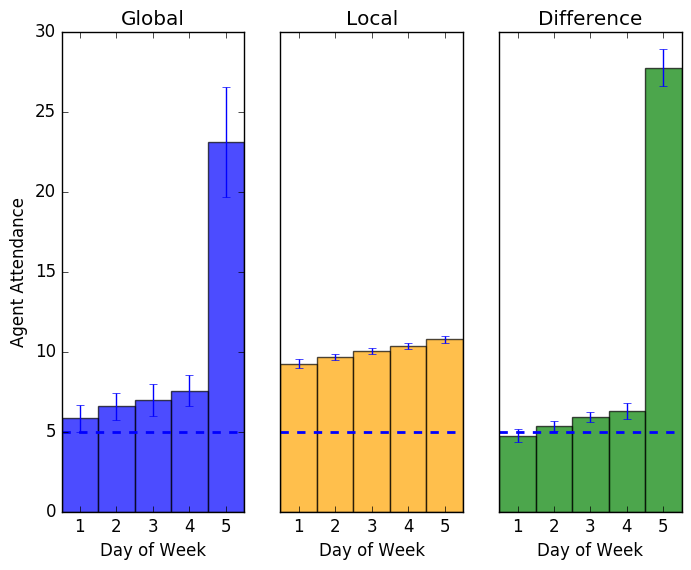
\includegraphics[width=0.45\textwidth]{Histograms0}
\caption{Attendance for Bar Problem for N=50, k=5, b=5}
\label{hist0}
\end{figure}

\begin{figure}[h]
\centering
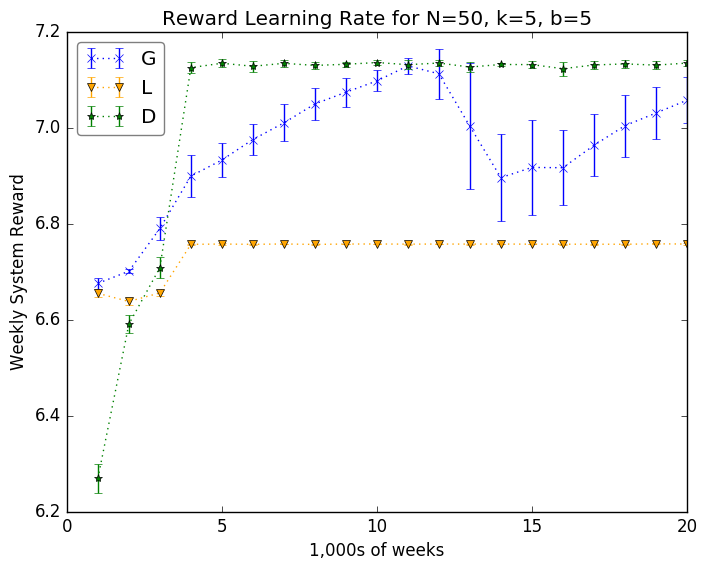
\includegraphics[width=0.45\textwidth]{Scatter0}
\caption{Reward for Bar Problem for N=50, k=5, b=5}
\label{scatter0}
\end{figure}

%Q-learning for scenario 1
For the Battle of Bars problem, simulations were run for 10,000 iterations. Each trial was ran 10 times and values were averaged over all trials.

\begin{figure}[ht]
\centering
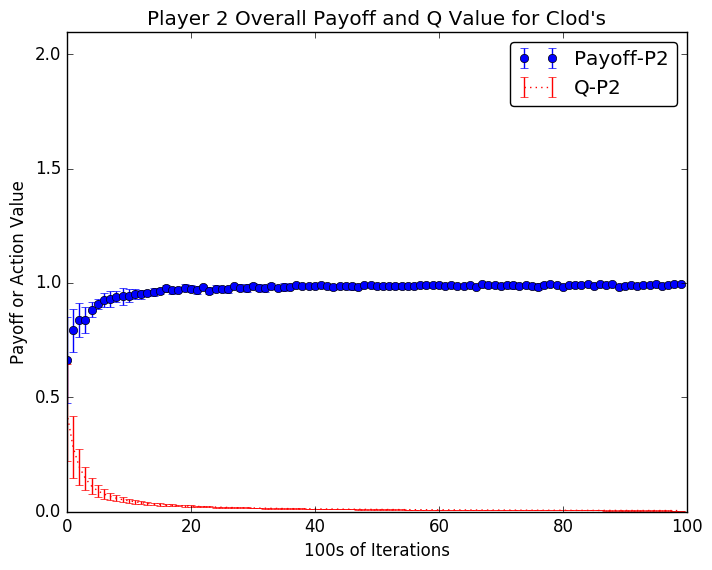
\includegraphics[width=0.45\textwidth]{Scenario1}
\caption{Reward and Action-Learner(Q) for Battle of the Bars where P1 always goes to McMenamin's}
\label{scenario1}
\end{figure}
%Q-learning for scenario 2
\begin{figure}[ht]
\centering
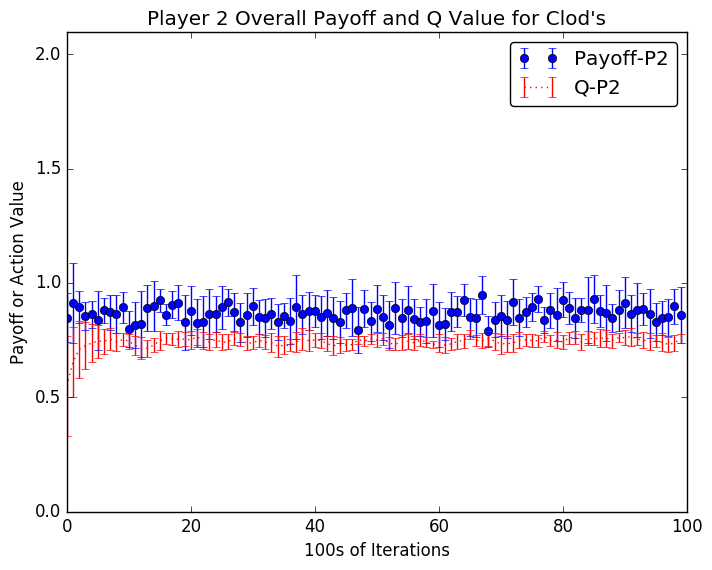
\includegraphics[width=0.45\textwidth]{Scenario2}
\caption{P2 Reward and Action-Learner(Q) for Battle of the Bars where P1 randomly chooses between the two bars}
\label{scenario2}
\end{figure}

\begin{figure}[ht]
\centering
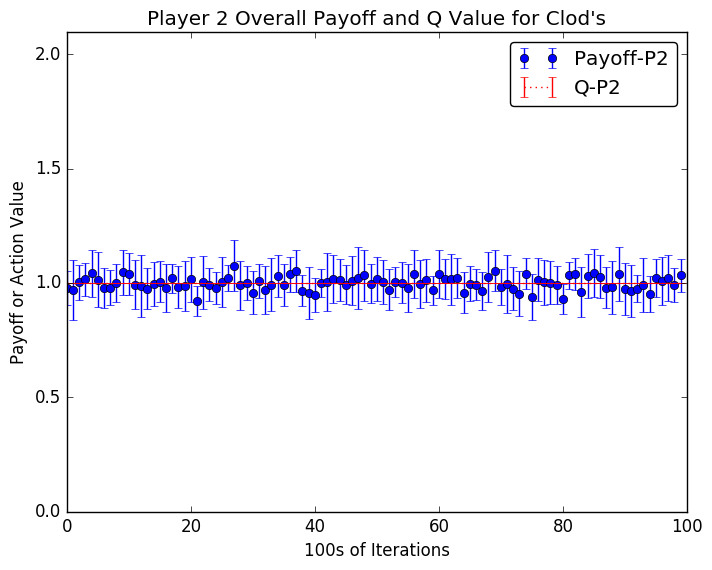
\includegraphics[width=0.45\textwidth]{Scenario2_optimal}
\caption{P2 Reward and Optimal Actions for Battle of the Bars where P1 randomly chooses between the two bars}
\label{scenario2_optimal}
\end{figure}

%Q-learning for scenario 3
\begin{figure}[ht]
\centering
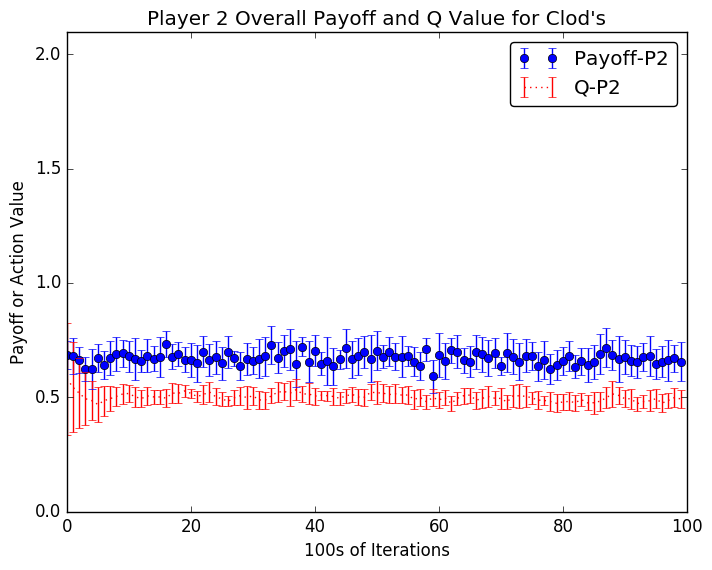
\includegraphics[width=0.45\textwidth]{Scenario3}
\caption{P2 Reward and Optimal Actions for Battle of the Bars where P1 favors Mcmenamin's 2/3 of the time}
\label{scenario3}
\end{figure}
%Q-learning for scenario 4
\begin{figure}[ht]
\centering
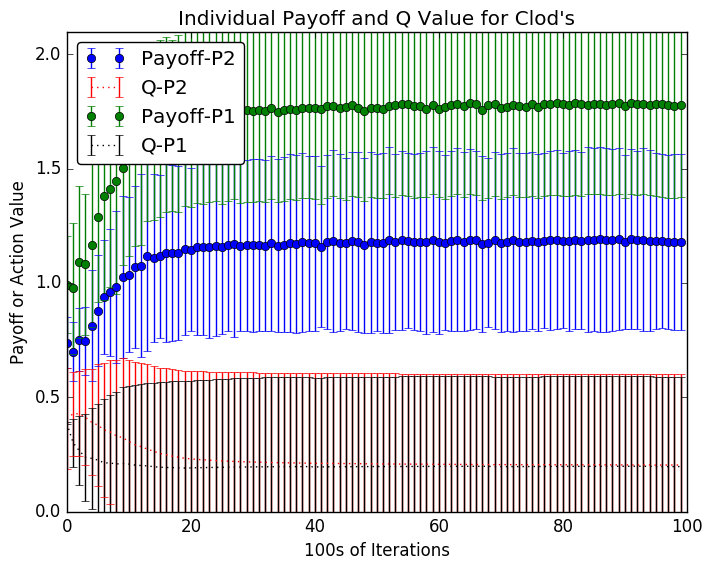
\includegraphics[width=0.45\textwidth]{Scenario4}
\caption{P2 Reward and Optimal Actions for Battle of the Bars when Agents Find Equilibrium through Simulation}
\label{scenario4}
\end{figure}

\begin{figure}[ht]
\centering
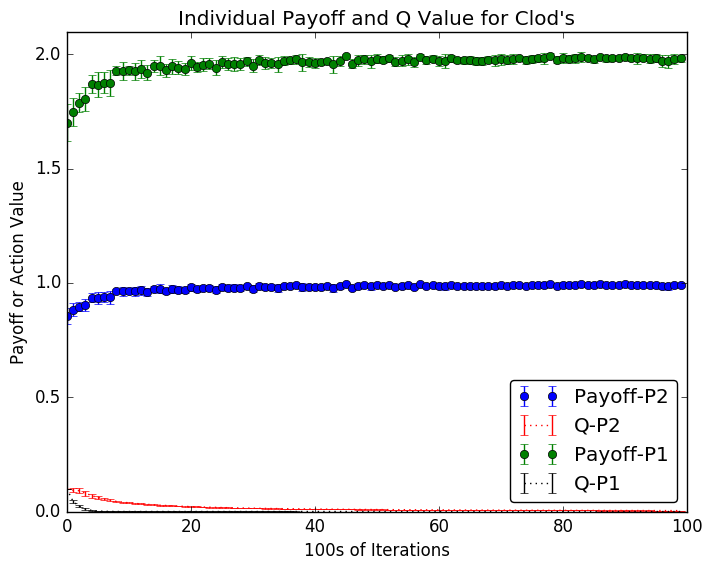
\includegraphics[width=0.45\textwidth]{Scenario4_seeded}
\caption{Both agent Reward and Optimal Actions for Battle of the Bars when Agents Find Equilibrium through Simulation}
\label{scenario4_seeded}
\end{figure}

\subsection{Analysis}
\subsubsection{BAR PROBLEM}

The local reward and the global reward produce different Nash equilibrium.  In the case with the local reward, the Nash equilibrium is for agents to evenly distribute.  If the distribution is $[10, 10, 10, 9, 11]$, an agent from the day with 11 people can unilaterally change their decision to achieve a higher reward.  The Nash Equilibrium for the local reward is $[10, 10, 10, 10, 10]$.

However, if the reward is the global reward, the Nash Equilibrium is $[5, 5, 5, 5, 30]$.  In this situation, the maximum reward for the system is to achieve optimal attendance on as many nights as possible.  No change in decision by a single agent can create a higher global reward.  There is no incentive for any agent to change their choice.  Between the global reward and the local reward, the local reward converges to a sub-optimal solution for the system as demonstrated in Figures \ref{hist0} and \ref{scatter0}.


The counterfactual reward provides an alternative method to reward the agents.  This method should reach the same equilibrium as the global reward. From the equilibrium $[5, 5, 5, 5, 30]$, the agents who are at the night with 30 total agents, receives a small negative reward.  However, if the agent were to attend a night with 5 people, they would receive a larger negative reward.  No agent can make a unilateral move to improve their reward.  The difference reward has the same Nash Equilibrium as the global reward

\subsubsection{BATTLE OF THE BARS}
If Player 1 only goes to McMenamin's, the only way for Player 2 to receive a reward is to go to the same bar.  If Player 2 chooses the other bar, she will not receive any reward.  This result is confirmed by a simple action value learner as seen in Figure \ref{scenario1}.  This set of actions is a Nash Equilibrium.  Neither agent can gain by deviating from their current action.

If Player 1 decides to soften and attend both bars with a 50\% probability, Player 2 can make a strategic decision to maximize her reward.  Because the two bars do not offer the same reward, Player 2 should attend Clod's more.  This is not confirmed by an action-learner simulation, but can be clearly seen in Figures \ref{scenario2} and  \ref{scenario2_optimal}.   The action-learner converges to an action profile of [0.75, 0.25].  This is not the best strategy.  A higher reward is achieved when P2 attends Clod's 100\% of the time.  This is not a Mixed Strategy Nash Equilibrium.  Player 1 can change her action profile to achieve a higher reward overall. The action learner has trouble converging to the proper solution because it continues to receive a reward for attending McMenamin's when Player 1 is present.  The value for not choosing Clod's will never go to zero.  That is why the learner settles on a non-optimal solution.

A third scenario is also investigated.  Player 1 begins to favor McMenamin's again.  She does so in a way that is proportional to the reward that she receives.  She will attend McMenamin's 2/3 of the time and Clod's 1/3 of the time. As a result, Player 2's action profile is independent of her reward.  For any action profile, Player 2's expected return will be the same.  The action-learner returns an action profile of [0.5, 0.5].  Both actions give the same weighted reward over the entire trial.  Although all values allow the agent to achieve the same payoff, only one set of values is the Nash Equilibrium if Player 1 maintains a [1/3, 2/3] action profile.  The Nash Equilibrium is when Player 2 has an action profile of [2/3, 1/3].  This will be seen in the next scenario.


The final scenario analyzed is to allow the agents to reach equilibrium on their own.

\begin{table}[ht]
\centering
\begin{tabular}{@{}cccc@{}}
\toprule
 & \multicolumn{3}{c}{Nash Equilibrium} \\
 & 1 & 2 & 3 \\
\begin{tabular}[c]{@{}c@{}}Player 1\\ Action Profile\end{tabular} & {[}1,0{]} & {[}0,1{]} & {[}1/3, 2/3{]} \\
\begin{tabular}[c]{@{}c@{}}Player 2\\ Action Profile\end{tabular} & {[}1,0{]} & {[}0,1{]} & {[}2/3, 1/3{]} \\
\begin{tabular}[c]{@{}c@{}}Player 1\\ Payoff\end{tabular} & 1 & 2 & 2/3 \\
\begin{tabular}[c]{@{}c@{}}Player 2\\ Payoff\end{tabular} & 2 & 1 & 2/3 \\ \bottomrule
\end{tabular}
\caption{All 3 Nash equilibrium and corresponding payoffs for players}
\label{nash_table}
\end{table}


As the previous scenarios have shown, when the agents have the action profiles in  Table \ref{nash_table}, any unilateral change in action by either agent will not produce a higher payoff.  The simulation pushes towards either of the first two equilibrium.  The third equilibrium will not appear in simulation because if one agent is at this point, the other has no incentive to stay.  Exploration will cause this agent to deviate from the point which will then cause the other agent to deviate.  This solution is basically at the top of a hill.  Any deviation causes a descent to one of the other solutions.  For the other two equilibrium points, as one agent approaches the pure strategy, the other agent must match this profile otherwise they will receive less of a payoff.  The simulation for \ref{scenario4} shows very large error bars.  The large error is caused by the agents converging to different equilibrium each trial.  Figure \ref{scenario4_seeded} shows that if the action learner is seeded for both agents such that the relative preferences are the same for each trial, convergence will occur toward the same equilibrium every time.  The payoff for both agents is less in the mixed Nash equilibrium compared to the pure strategies.  Payoffs for each equilibrium can be seen in Table \ref{nash_table}.  The mixed strategy equilibrium is not Pareto optimal and does not maximize a total sum welfare.


\end{document}
